\subsection{Active material at a wall between absorbing phases}
\label{sec:wall}

A wall separating the all-alive and all-dead phases creates an active
layer without preparing an active region initially. We measure the
interface sites per unit wall length, $I=L_y\iota/2$, and subtract the
matched $q=0$ baseline to obtain excess adsorption $\Gamma=I-I_0$.
At $L_y=8192$, $L_x=16384$, four runs per point give
$\Gamma=133.27$, 166.15 and 190.86 at $q=0.04584$, 0.04588 and
0.04590 over $5$--$10\times10^6$ steps
(Fig.~\ref{fig:gpu_wetting}). The shorter walls, $L_x=4096$, give
134.80, 168.37 and 199.90. The closest point therefore retains a size
effect of about 4.5\%; each of the four longer-wall runs also declines
slightly between halves of the late window.

\begin{figure*}
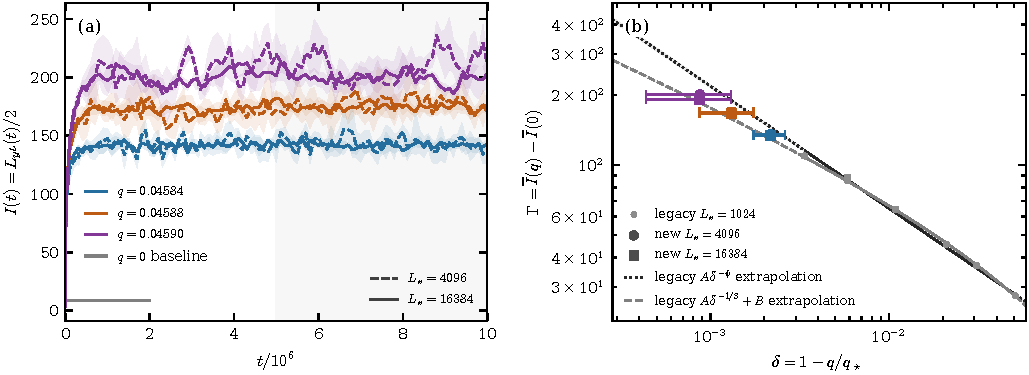
\includegraphics[width=\textwidth]{figs/fig_gpu_wetting}
\caption{Extended wall trajectories at $p=\alpha=1/2$, $L_y=8192$,
and $L_x=4096$ or 16384. Each nonzero-$q$ group contains four independent
runs to $10^7$ steps; each matching $q=0$ baseline contains two runs to
$2\times10^6$. (a) Interface sites per unit wall length. Line styles
distinguish $L_x$, and shading gives pointwise 95\% run-bootstrap
intervals. The gray span marks the $5$--$10\times10^6$ averaging window.
(b) Excess adsorption relative to the matched baseline. Vertical
intervals include shared-baseline sampling uncertainty; horizontal bars
show coexistence-reference sensitivity. Gray points and both
two-parameter fits use only the seven earlier $L_x=1024$ points.
Dashed and dotted continuations are predictions for the new data, with
conditional parameter-bootstrap bands at $q^*=0.04594$. These bands
exclude reference sensitivity and size/time systematics. No exponent is
fitted to the new data.}
\label{fig:gpu_wetting}
\end{figure*}


Increasing adsorption is consistent with a thickening active film, but
also depends on the activity inside the film. The existing measurements
establish neither divergence of the edge separation nor a wetting
exponent. Two-parameter fits to the earlier seven-point data, a pure
power and a one-third power with an additive offset, do not jointly
describe the new points within their sampling errors. Size, time,
and front-reference sensitivity remain visible
(Supplemental Sec.~\ref{S-sec:swall}).
Equilibrium complete wetting in two dimensions supplies a useful
comparison~\cite{lipowsky1983,fisher1984,carlon1999}, and active boundary
layers also occur between defensive alliances~\cite{szabo2007}.
Here a theory must describe the interaction of two fluctuating
active--absorbing fronts.
